\documentclass[10pt]{article}         %% What type of document you're writing.

%%%%% Preamble

%% Packages to use

\usepackage{amsmath,amsfonts,amssymb,mathtools}   %% AMS mathematics macros
\usepackage{graphicx}
\usepackage{caption}
\usepackage{subcaption}
\usepackage{tikz}
\usetikzlibrary{decorations.pathreplacing,matrix}
\usetikzlibrary{decorations.pathmorphing}
\usetikzlibrary{decorations.text}

\tikzset{ 
  table/.style={
    matrix of math nodes,
    row sep=-\pgflinewidth,
    column sep=-\pgflinewidth,
    nodes={rectangle,text width=3em,align=center},
    text depth=1.0ex,
    text height=1.0ex,
    nodes in empty cells,
    left delimiter=[,
    right delimiter={]},
  }
}

\DeclarePairedDelimiter\abs{\lvert}{\rvert}%
\DeclarePairedDelimiter\norm{\lVert}{\rVert}%
\newtheorem{exmp}{Example}[section]
%% Title Information.

\title{Visual Odometry sparse bundle adjustment and feature uncertainty}
\author{Ilan Shimshoni, Ehud Rivlin, Alex Kreimer}

\begin{document}

\maketitle

\section{Notation and problem statement}

This section makes definitions that are used throughout the document.

Let the camera $j$ be parameterized by a vector $a_j$, $j=1,\dotsc,n$,
and 3d the point $i$ by vector $b_i$, $i=1,\dotsc,m$.  We assume
calibrated cameras and thus parameterize only the extrinsic camera
parameters.  The rotation is represented by three Euler angles and the
translation is taken ``as is''. \emph{Parameter} vector
$\theta\in R^M$ is defined as:
$\theta=[a_1^T,\dotsc,a_n^T,b_1^T, \dotsc,b_m^T]^T$.

$x_{ij}\in\mathcal{R}^k$ denotes the image coordinates 3d point $i$ as
seen in image $j$.

\emph{Measurement} vector is defined by image observations:
$X = [x_{11}^T,\dotsc, x_{1m}^T,\allowbreak
x_{21}^T,\dotsc,x_{2m}^T,\dotsc,x_{n1}^T,\dotsc,x_{nm}^T]$,
$X\in\mathcal{R}^N$ and it is accompanied by its covariance data
$\Sigma_X=diag(\Sigma_{x_{11}},\dotsc,\Sigma_{x_{nm}})$,
$\Sigma_{ij}\in \mathcal{R}^{k\times k}$. In case of missing
measurement it just disappears from the measurement vector, so the
indices may have ``holes'' in them.

\emph{Prediction} vector is a function of the parameter vector $\theta$:
$\hat{X} = [\hat{x}_{11}^T,\dotsc,\hat{x}_{1m}^T,\allowbreak
\hat{x}_{21}^T,\dotsc,\allowbreak
\hat{x}_{2m}^T,\dotsc,\hat{x}_{n1}^T,\dotsc,\hat{x}_{nm}^T]$,
s.t. $\hat{x}_{ij} =f_{ij}(P)$.

Bundle adjustment is problem of finding a set of parameters that make
observations in different views as ``consistent'' as possible.

\subsection{Sparse BA}
The following definitions are relevant for the sparse implementation
of the BA and are not used in other sections of this document. 

Let
$A_{ij}= \frac{\partial \hat{x}_{ij}}{\partial a_j}\in
\mathcal{R}^{k\times \text{size}(a)}$,
$B_{ij}= \frac{\partial \hat{x}_{ij}}{\partial b_i}\in
\mathcal{R}^{k\times \text{size}(b)}$.
The Jacobian of the prediction is
$J=[\partial \hat{X}/\partial a\ \partial \hat{X}/\partial b]=[A\ B]$.
Note that
$\frac{\partial \hat{x}_{ij}}{\partial a_k}=0, \forall j\neq k$ and
that $\frac{\partial \hat{x}_{ij}}{\partial b_k}=0, \forall i\neq k$.

This special structure of the Jacobian allows to perform a more
efficient optimization (LM) procedure.

\subsection{Problem Formulation}

\subsubsection{Maximum Likelihood}

Maximum likelihood estimator seeks to maximize the likelihood of the
data given the parameters:
\[
\theta_{ML} = \underset{\theta}{\text{argmax}}\ p(X|\theta)
\]
We assume that the measurements adhere to the following statistical
model:
\[
x_{ij} = \hat{x}_{ij}+\epsilon_{ij}
\]
where $\hat{x}_{ij}$ is the model prediction, $\epsilon_{ij}$ is a
Gaussian noise with zero mean and a known covariance
$\Sigma_{ij}$. Thus $x_{ij}$ is a $k$-vector Gaussian random variable
with mean $\hat{x}_{ij}$ and covariance matrix $\Sigma_{ij}$. Hence
the probability density of $x_{ij}$ given $\theta$ is:
\[
p(x_{ij}|\theta)=\frac{1}{\sqrt{(2\pi)^n\left|\Sigma_{ij}\right|}}\exp^{-(x_{ij}-\hat{x}_{ij},\Sigma_{ij}^{-1}(x_{ij}-\hat{x}_{ij}))/2}
\]

Thus ML estimator is:
\[
\theta_{ML} = \underset{\theta}{\text{argmax}}\ p(X|\theta) =
\underset{\theta}{\text{argmax}} \prod_{i,j} p(x_{ij}|\theta)
=\underset{\theta}{\text{argmin}}\ \sum_{ij}\left\| x_{ij}-\hat{x}_{ij}\right\|_{\Sigma_{ij}}
\]

This is typical formulation of BA procedure found in the
literature. 

\emph{Note}: if the covariances are all of the form $\Sigma_{ij}=a I$
then
\[
\underset{\theta}{\text{argmin}}\ \sum_{ij}\left\|
  x_{ij}-\hat{x}_{ij}\right\|_{\Sigma_{ij}} = \underset{\theta}{\text{argmin}}\ \sum_{ij}\left\|
  x_{ij}-\hat{x}_{ij}\right\|_2^2
\]
thus minimization of unweighted reprojection errors implicitly assumes
equal measurement covariance.

\subsubsection{Maximum a posteriori probability}

Now we assume a joint distribution $p(X,\theta)$ and seek to maximize
the posterior distribution on the parameters
\[
\theta_{MAP} = \underset{\theta}{\text{argmax}}\ p(\theta|X)= \underset{\theta}{\text{argmax}}\ p(X|\theta)p(\theta)
\]

In case of a Gaussian zero mean and a known covariance  prior over the parameters
\[
\theta_{MAP} = \underset{\theta}{\text{argmin}}\ \sum_{ij}\left\|
  x_{ij}-\hat{x}_{ij}\right\|_{\Sigma_{ij}} + \sum_i
\left\|b_i-b_i^0\right\|_{\Sigma_{b_i}} + \sum_j\left\|a_j-a_j^0\right\|_{\Sigma_{a_j}}
\]
\emph{Note} Motion priors may be modelled as a distribution over
the camera extrinsic parameters while structure uncertainty may be
modeled as a prior distribution over the structure parameters.

\subsection{Parameterization}

3d points are represented by 3 vectors $b_j = X_j = [X_j,Y_j,Z_j]^T$.
Camera motion is parameterized by a 6 vector
$a_i = [r_x,r_y,r_z,t_x,t_y,t_z]$.  Rotations are parameterized using
Euler angles $ R = R_z(r_z)R_y(r_y)R_x(r_x)$.  Translation is
represented by a 3 vector $ dt = [d_x,d_y,d_z]^T$. Left (right) camera
$i$ projection of 3d point $X_j$:
$$
\begin{aligned}
  \hat{x}^{(l)}_{ij} &= \pi^{(l)}(a_i,b_j) = K[R^{(l)}(a_i)\ T^{(l)}(a_i)]b_j\\
  \hat{x}^{(r)}_{ij} &= \pi^{(r)}(a_i,b_j) = K[R^{(r)}(a_i)\
  T^{(r)}(a_i)]b_j
\end{aligned}
$$

\section{Sparse LM for bundle adjustment}

We use sparse LM algorithm to solve ~\ref{eq:prob}. The algorithm
exploits the fact that feature point coordinates in view $i$ depend
only on the parameters of view $i$, which gives the Jacobian a special
sparse structure.



LM (dampered) normal equations are:
$$
(J^T\Sigma^{-1}_XJ+\lambda I)\delta = -J^T\Sigma^{-1}_X\epsilon
$$
\begin{exmp} Below we show the structure of the Jacobian in case $n=3$
  views, $m=4$ 3d points.
  \begin{equation}\label{eq:sparsej}
    J=\frac{\partial \hat{X}}{\partial P} = 
    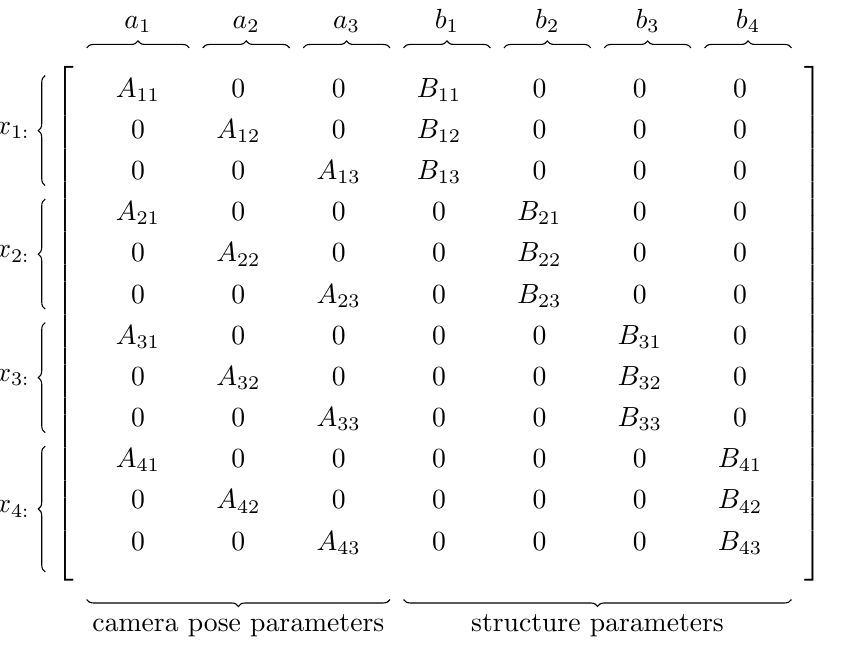
\begin{tikzpicture}[baseline,decoration=brace]
      \matrix (J) [table] {
        A_{11} &0 &0 &B_{11} &0 &0 &0\\
        0 &A_{12} &0 &B_{12} &0 &0 &0\\
        0 &0 &A_{13} &B_{13} &0 &0 &0\\
        A_{21} &0 &0 &0 &B_{21} &0 &0\\
        0 &A_{22} &0 &0 &B_{22} &0 &0\\
        0 &0 &A_{23} &0 &B_{23} &0 &0\\
        A_{31} &0 &0 &0 &0 &B_{31} &0\\
        0 &A_{32} &0 &0 &0 &B_{32} &0\\
        0 &0 &A_{33} &0 &0 &B_{33} &0\\
        A_{41} &0 &0 &0 &0 &0 &B_{41}\\
        0 &A_{42} &0 &0 &0 &0 &B_{42}\\
        0 &0 &A_{43} &0 &0 &0 &B_{43}\\
      }; \draw [decorate,transform canvas={yshift=1em}] (J-1-1.north
      west) --
      node[above=2pt]{$a_1$} (J-1-1.north east); \draw
      [decorate,transform canvas={yshift=1em}] (J-1-2.north west)
      ++(.2,0) --
      node[above=2pt]{$a_2$} (J-1-2.north east); \draw
      [decorate,transform canvas={yshift=1em}] (J-1-3.north west)
      ++(.2,0) --
      node[above=2pt]{$a_3$} (J-1-3.north east); \draw
      [decorate,transform canvas={yshift=1em}] (J-1-4.north west)
      ++(.2,0) --
      node[above=2pt]{$b_1$} (J-1-4.north east); \draw
      [decorate,transform canvas={yshift=1em}] (J-1-5.north west)
      ++(.2,0) --
      node[above=2pt]{$b_2$} (J-1-5.north east); \draw
      [decorate,transform canvas={yshift=1em}] (J-1-6.north west)
      ++(.2,0) --
      node[above=2pt]{$b_3$} (J-1-6.north east); \draw
      [decorate,transform canvas={yshift=1em}] (J-1-7.north west)
      ++(.2,0) -- node[above=2pt]{$b_4$} (J-1-7.north east);
  
      \draw [decorate,decoration=mirror,transform
      canvas={yshift=-1em}] (J-12-1.south west) --
      node[below=2pt]{camera pose parameters} (J-12-3.south east);
      \draw [decorate,decoration=mirror,transform
      canvas={yshift=-1em}] (J-12-4.south west) ++(.2,0) --
      node[below=2pt]{structure parameters} (J-12-7.south east);

      \draw [decorate,transform canvas={xshift=-1.5em}] (J-3-1.south
      west) ++(0,.2)-- node[left=2pt]{$x_{1:}$} (J-1-1.north west);
      \draw [decorate,transform canvas={xshift=-1.5em}] (J-6-1.south
      west) ++(0,.2) -- node[left=2pt]{$x_{2:}$} (J-4-1.north west);
      \draw [decorate,transform canvas={xshift=-1.5em}] (J-9-1.south
      west) ++(0,.2)-- node[left=2pt]{$x_{3:}$} (J-7-1.north west);
      \draw [decorate,transform canvas={xshift=-1.5em}] (J-12-1.south
      west) -- node[left=2pt]{$x_{4:}$} (J-10-1.north west);

    \end{tikzpicture}
  \end{equation}

  Note that it is possible to change the order of elements in the
  measurement vector and to obtain a bit different sparse structure
  which is described in the appendix of \cite{Zisserman}.


  \textbf{Note (TBD)}: Let
  $\hat{x}_{11} = [h2e(P^{(l)}_1b_1)^T,h2e(P^{(r)}_1b_1)^T]^T$ and
  $\hat{x}_{21} = [h2e(P^{(l)}_1b_2)^T,h2e(P^{(r)}_1b_2)^T]^T$. The
  dependence of $ \frac{\partial x_{11}}{\partial b_1}$ on $b_1$ is
  because of h2e, so if we can use homogenious coordinates instead of
  eucledian, most of the $B_{ij}$ will be the same.

  If we substitute ~\ref{eq:sparsej} into $J^T\Sigma^{-1}_XJ$ and use
  these assignments:
  \begin{equation}
    U_j = \sum_{i=1}^4A_{ij}^T\Sigma_{x_{ij}}^{-1}A_{ij};\ V_i= \sum_{j=1}^3B_{ij}^T\Sigma_{x_{ij}}^{-1}B_{ij};\ W_{ij}= A_{ij}^T\Sigma_{x_{ij}}^{-1}B_{ij} 
  \end{equation}
  we get
  \begin{equation}
    J^T\Sigma^{-1}_XJ = 
    \begin{bmatrix}
      U_1 &0 &0 &W_{11} &W_{12} &W_{13} &W_{14}\\
      0 &U_2 &0 &W_{21} &W_{22} &W_{23} &W_{24}\\
      0 &0 &U_3 &W_{31} &W_{32} &W_{33} &W_{34}\\
      W_{11}^T &W_{12}^T &W_{13}^T &V_1 &0 &0 &0\\
      W_{21}^T &W_{22}^T &W_{23}^T &0 &V_2 &0 &0\\
      W_{31}^T &W_{32}^T &W_{33}^T &0 &0 &V_3 &0\\
      W_{41}^T &W_{42}^T &W_{43}^T &0 &0 &0 &V_4\\
    \end{bmatrix}
  \end{equation}
  Letting
  \begin{equation}
    \epsilon_{a_j}=\sum_{i=1}^4A_{ij}^T\Sigma_{X_{ij}}^{-1}\epsilon_{ij},\ \epsilon_{b_i}=\sum_{j=1}^3B_{ij}^T\Sigma_{X_{ij}}^{-1}\epsilon_{ij},\ \text{with}\ \epsilon_{ij} = x_{ij}-\hat{x}_{ij}
  \end{equation}

\begin{equation}
  J^T\Sigma^{-1}_XJ\delta = -J^T\Sigma^{-1}_X\begin{pmatrix}\epsilon_a\\ \epsilon_b\end{pmatrix}
\end{equation}
becomes
\begin{equation}
  \begin{bmatrix}
    U_1 &0 &0 &W_{11} &W_{12} &W_{13} &W_{14}\\
    0 &U_2 &0 &W_{21} &W_{22} &W_{23} &W_{24}\\
    0 &0 &U_3 &W_{31} &W_{32} &W_{33} &W_{34}\\
    W_{11}^T &W_{12}^T &W_{13}^T &V_1 &0 &0 &0\\
    W_{21}^T &W_{22}^T &W_{23}^T &0 &V_2 &0 &0\\
    W_{31}^T &W_{32}^T &W_{33}^T &0 &0 &V_3 &0\\
    W_{41}^T &W_{42}^T &W_{43}^T &0 &0 &0 &V_4\\
  \end{bmatrix}
  \begin{bmatrix}
    \delta_{a_1}\\ \delta_{a_2}\\ \delta_{a_3}\\ \delta_{b_1}\\
    \delta_{b_2}\\ \delta_{b_3}\\ \delta_{b_4}
  \end{bmatrix}
  =
  \begin{bmatrix}
    \epsilon_{a_1}\\ \epsilon_{a_2}\\ \epsilon_{a_3}\\
    \epsilon_{b_1}\\ \epsilon_{b_2}\\ \epsilon_{b_3}\\ \epsilon_{b_4}
  \end{bmatrix}
\end{equation}
\end{exmp}
In general case (* denotes LM augmentation):
\begin{equation}
  \begin{pmatrix}
    U^*& W\\
    W^T& V^*
  \end{pmatrix}
  \begin{pmatrix}\delta_a\\ \delta_b\end{pmatrix} = \begin{pmatrix}\epsilon_a\\ \epsilon_b\end{pmatrix}
\end{equation}
We premultiply by
\begin{equation}
  \begin{pmatrix}
    I &-WV^{*-1}\\
    0 &I
  \end{pmatrix}
\end{equation}
and thus obtain:
\begin{equation}
  \begin{pmatrix}
    U^*-WV^{*-1}W^T& 0\\
    W^T& V^*
  \end{pmatrix}
  \begin{pmatrix}\delta_a\\ \delta_b\end{pmatrix} = 
  \begin{pmatrix}\epsilon_a - WV^{*-1}\epsilon_b\\ \epsilon_b\end{pmatrix}
\end{equation}


\section{Representation of rotation}
\label{sec: rot_mat}
We use Euler angles to parameterize the rotation $\mathbf{r} = [r_x,r_y,r_z]$. To simplify the formulas we adopt this notation:
\begin{align*}
  c_x &= cos(r_x) & c_y &= cos(r_y) & c_z&=cos(r_z) \\
  s_x &= sin(r_x) & s_y &= sin(r_y) & s_z&=sin(r_z)
\end{align*}
Elementary rotation matrices are:
\begin{align*}
R_x&= R(r_x) = 
\begin{bmatrix}
1& 0& 0\\
0& c_x& -s_x\\
0& s_x& c_x
\end{bmatrix} & R_y&=R_y(r_y) = \begin{bmatrix}
c_y& 0& s_y\\
0& 1& 0\\
-s_y& 0& c_y
\end{bmatrix} &R_z &= R_z(r_z) = \begin{bmatrix}
c_z& -c_z& 0\\
c_z& c_z& 0\\
0& 0& 1
\end{bmatrix}
\end{align*}
Rotation matrix parameterized by $\mathbf{r}$ is:
\[
R(\mathbf{r}) = R_xR_yR_z =
\begin{bmatrix}
 +c_yc_z& -c_ys_z& +s_y\\
 +s_xs_yc_z+c_xs_z& -s_xs_ys_z+c_xc_z& -s_xc_y\\
 -c_xs_yc_z+s_xs_z& +c_xs_ys_z+s_xc_z& +c_xc_y\\
\end{bmatrix}
\]
\subsection{Central projection}
3d point $X_i = (X,Y,Z,1)^T$ is measured in coordinate system $O_1$.  The camera is located at the origin of the coordinate system $O_2$.  Rigid transformation parameterized by $\mathbf{r,t}$ transforms $X_i$ into $O_2$.  Thus a central projection of a transformed 3d point is given by:
$$
\pi_h(\mathbf{r,t}) =\begin{bmatrix} u\\v\\l \end{bmatrix} =  K\Big[R(\mathbf{r}), \mathbf{t}\Big]X_i\\
$$
\begin{align*} &=
  \begin{bmatrix} f& 0& c_u\\ 0& f& c_v\\0& 0& 1\\ \end{bmatrix}
  \begin{bmatrix}
    +c_yc_z& -c_ys_z& +s_y & t_x\\
    +s_xs_yc_z+c_xs_z& -s_xs_ys_z+c_xc_z& -s_xc_y & t_y\\
    -c_xs_yc_z+s_xs_z& +c_xs_ys_z+s_xc_z& +c_xc_y & t_z\\
    0 & 0 & 0 & 1\\
  \end{bmatrix}
  \begin{bmatrix}X\\Y\\Z\\1\end{bmatrix}\\
    &= \begin{bmatrix} f& 0& c_u\\ 0& f& c_v\\0& 0& 1\\ \end{bmatrix}
    \begin{bmatrix}
      Xc_yc_z-Yc_ys_z+Zs_y+t_x\\
      Xs_xs_yc_z+Xc_xs_z-Ys_xs_ys_z+Yc_xc_z-Zs_xc_y+t_y\\
      -Xc_xs_yc_z+Xs_xs_z+Yc_xs_ys_z+Ys_xc_z+Zc_xc_y+t_z\\
    \end{bmatrix}\\
    &=\begin{bmatrix}
      f(Xc_yc_z-Yc_ys_z+Zs_y+t_x)+c_u(-Xc_xs_yc_z+Xs_xs_z+Yc_xs_ys_z+Ys_xc_z+Zc_xc_y+t_z)\\
      f(Xs_xs_yc_z+Xc_xs_z-Ys_xs_ys_z+Yc_xc_z-Zs_xc_y+t_y)+c_v(-Xc_xs_yc_z+Xs_xs_z+Yc_xs_ys_z+Ys_xc_z+Zc_xc_y+t_z)\\
      -Xc_xs_yc_z+Xs_xs_z+Yc_xs_ys_z+Ys_xc_z+Zc_xc_y+t_z\\
    \end{bmatrix}\\
\end{align*}
\end{document}

%%% Local Variables:
%%% mode: latex
%%% TeX-master: t
%%% End:
